\chapter{Metadata Evolution and Verification}

\section{Verication through Sensor Data}

\section{Types of Verification}
\subsection{Geometric Verification}
\subsection{Functional Verification}
\subsection{Value Verification}

\section{Structural Verification With Empirical Mode Decomposition}

\section{Problem description}
\begin{figure}
\begin{center}
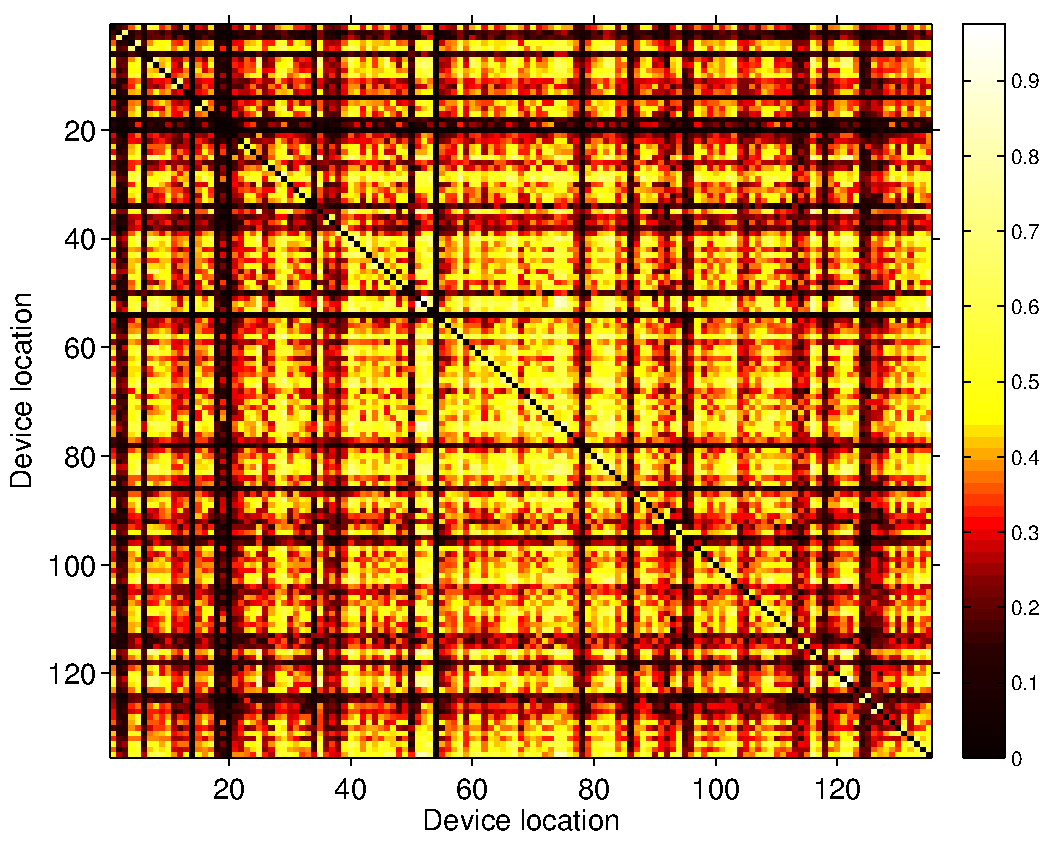
\includegraphics[width=.5\textwidth]{figs/heatMap_raw_201106-eps-converted-to.pdf}
\caption{Correlation coefficients of the raw traces from the Building 1 dataset (Section \ref{data:engbldg2}).
The matrix is ordered such as the devices serving same/adjacent rooms are nearby in the matrix.}
\label{fig:heatmap:raw}
\end{center}
\end{figure}

The primary objective of SBS is to determine \emph{how} device usage patterns are correlated across all pairs of sensors and 
discover when these relationships change.  
The naive approach is to run correlation analysis on pairs of sensor traces, recording their correlation coefficients over time and 
examining when there is a statistically-significant deviation from the norm.  
However, this approach does not yield any useful information when applied to \emph{raw data traces}.
For example, the two raw signals shown in Figure~\ref{fig:diagram1} are from two independent HVAC systems,
 serving different rooms on different floors.
Since each space is independently controlled, we expect their power-draw signals to be uncorrelated (or at least distinguishable 
from other signal pairs).  However, their correlation coefficient ($0.57$), is not particularly informative -- it is statistically
similar to the correlation between itself and other signals in the trace.  
  
Using a larger set of devices, Figure \ref{fig:heatmap:raw} shows a correlation matrix with 135 distinct lighting and HVAC systems serving numerous rooms in a building (described later on in Section \ref{data:engbldg2}).
The indices are selected such that their index-difference is indicative of their relative spatial proximity.  
For example, a device in location 1 is closer in the building to a device in location 2 than it is to 
a device in location 135. 
The color of the cell is the average pairwise correlation coefficient for devices in the row-column index.  The higher the value, the lighter the color.
Devices serving the same room are along the diagonal.  Because these devices are used simultaneously, we expect
high average correlation scores, lighter shades, along the diagonal figure.
However, we observe no such pattern.  %structure is unseen in the Figure.  
Most of the signals are correlated with all the others and we see no discernible structure.

\begin{figure}[t!]
\begin{center}
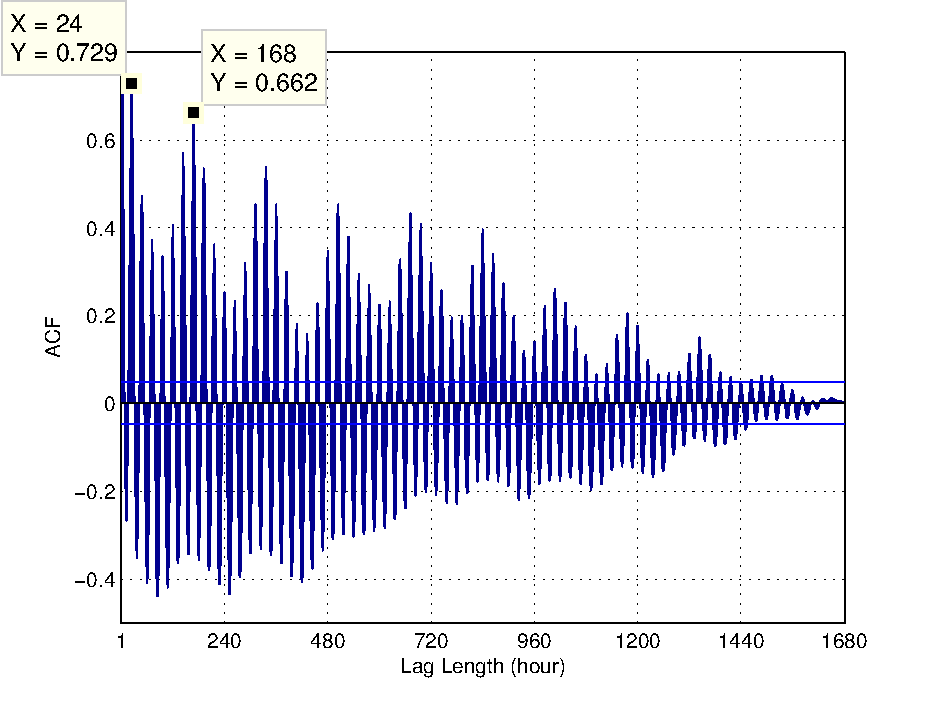
\includegraphics[width=.5\textwidth]{figs/acf_101A1_GHP-eps-converted-to.pdf}
\caption{Auto-correlation of a usual signal from the Building 1 dataset.
The signal features daily and weekly patterns (resp. $x=24$ and $x=168$).}
\label{fig:autocorr}
\end{center}
\end{figure}

An explanation for this is that the daily occupant usage patterns %office hours, 
drive these results.
Figure \ref{fig:diagram1} demonstrates this more clearly.  It shows two 1-week raw signals traces which feature the same 
diurnal pattern.  
This trend is present in almost every sensor trace, and, it hides 
the smaller fluctuations providing more specific patterns driven by local occupant activity.  Upon deeper inspection, we uncovered several
 dominant patterns, common among energy-consuming devices in buildings~\cite{wrinch:pes2012}.  Figure~\ref{fig:autocorr} depicts the 
 auto-correlation of a usual electric power signal for a device.  The two highest values in the figure correspond to a lag of 24 hours and 168 hours (one week).  
 Therefore, the signal has some periodicity and similar (though not equal) values are seen at daily and weekly time scales.
The daily pattern is due to daily office hours and the weekly pattern corresponds to weekdays and weekends.  
%Indeed, thorough inspection of the data reveals that the 
Correlation analysis on \emph{raw} signals cannot be used to determine meaningful 
inter-device relationships because periodic components act as non-stationary trends for high-frequency phenomenon, 
 making the correlation function irrelevant.  %metric is insufficient with raw signals containing the same dominant pattern.
Such trends must be removed in order to make meaningful progress towards our aforementioned goals.  

In the next section we describe SBS.  
We discuss \emph{strip and bind} in section~\ref{methodo:est}, which addresses de-trending and
relationship-discovery.  Then, we describe how we \emph{search} for changes in usage patterns, 
in section~\ref{methodo:ano}, to identify potential savings opportunities.








\section{Functional Verification through Classification and Experimentation}

\section{Value-Based Verification Through Physical-Model Checking}

\section{Related Work}

The research community has addressed the detection of abnormal energy-consumption in buildings in numerous ways \cite{katipamula:1review2005,katipamula:2review2005}. 

The rule-based techniques rely on a priori knowledge, they assert the sustainability of a system by identifying a set of undesired behaviors.
Using a hierarchical set of rules, Schein et al.\ propose a method to diagnose HVAC systems \cite{schein:hvacr2006}.
In comparison, state machine models take advantage of historical training data and domain knowledge to learn the states and transitions of a system.
The transitions are based on measured stimuli identified through a domain expertise.
State machines can model the operation of HVAC systems \cite{patnaik:toist2011} and permit to predict or detect the abnormal behavior of HVAC's components \cite{bellala:buildsys2012}.
However, the deployment of these methods require expert knowledge and are mostly applied to HVAC systems.

In~\cite{seem:energybldg2007}, the authors propose a simple unsupervised approach to monitor the average and peak daily consumption of a building and uncover outlier, nevertheless, the misbehaving devices are left unidentified.

Using regression analysis and weather variables the devices energy-consumption is predicted and abnormal usage is highlighted.
The authors of~\cite{brown:buildperf2012} use kernel regression to forecast device consumption and devices that behave differently from the predictions are reported as anomalous.
Regression models are also used with performances indices to monitor the HVAC's components and identify inefficiencies \cite{zhou:wiley2009}.
The implementation of these approaches in real situations is difficult, since it requires a training dataset and non-trivial 
parameter tuning.

Similar to our approach, previous studies identify abnormal energy-consumption using frequency analysis and unsupervised anomaly detection methods.
The device's consumption is decomposed using Fourier transform and outlier values are detected using clustering 
techniques \cite{Bellala_buildsys11,wrinch:pes2012,chen:aaaiw2011}. %jakkula
However, these methods assume a constant periodicity in the data and this causes many false positives in alarm reporting.  %, thus, they report devices usages happening at unusual times although they may not correspond to a faulty operation.
We do not make any assumption about the device usage schedule.  We only observe and model device relationships.
We take advantage of a recent frequency analysis technique that enables us uncover the inter-device relationships~\cite{romain:iotapp12}.
The identified anomalies correspond to devices that deviate from their normal relationship to other devices.

Reducing a building's energy consumption has also received a lot of attention from the research community.
% Since HVACs are one of the major electricity consumer in the buildings, several researchers have mainly focused on reducing the consumption of HVACs.
The most promising techniques are based on occupancy model predictions as they ensure that empty rooms are not over conditioned needlessly.
Room occupancy is usually monitored through sensor networks \cite{agarwal:ipsn2011,erickson:ipsn2011} or the computer network traffic \cite{kim:buildsys2010}.
These approaches are highly effective for buildings that have rarely-occupied rooms (e.g. conference room) and studies show that such approaches
 can achieve up to 42\% annual energy saving.
% However, these occupancy model predictions track human activity through sensor networks that usually imply the extra cost and privacy concerns.
SBS is fundamentally different from these approaches.  SBS identifies the abnormal usage of any devices rather than optimizing the normal usage of specific devices.
Nevertheless, the two approaches are complementary and energy-efficient buildings should take advantage of the synergy between them.






% Therefore, it is a practical way of reducing the energy consumption of any building in contrast to the anomaly detectors based on neural networks or kernel regression that requires training datasets and complex parameter tuning \cite{brown:buildperf2012}.
% Also, the proposed method does not require extra deployments such as sensors monitoring the room occupancy \cite{agarwal:ipsn2011,erickson:ipsn2011} or extra measurements for occupancy models (e.g. network traffic).
% 
% 
% This approach provides new insights in buildings energy consumption as it is fundamentally different from past works.
% complementary to other methods decreasing the energy consumption of the building normal operations.
% 
% it is more general (not only HVAC)
% 
% TODO look at IPSN TPC papers. Andreas Krause?

% 
% problem:
% The building energy consumption is mainly driven by its occupancy.
% The human occupancy is responsible for the majority of the devices energy consumption.
% For example, workstations, lights and air conditioners are utilized the most when humans occupied the building.
% 
% Thereby, all devices follow the same trend which is conducted by the human occupancy.
% In practice sensors data look all same.
% All devices are used during office hours and left off at night. (TODO see figure...)
% For our purpose, finding devices used simultaneously, this data is really difficult to analyze as the differences between each device is insignificant.
% 
% Our approach consists of; (1) subtract from the data the general trend driven by the building occupancy, (2) analyze remaining data to cluster devices used in concert.
% 
% 
% 
% result summary:
% We evaluate the proposed correlation estimator using 10 weeks of data from 135 devices serving 231 rooms.
% 
% contributions
% and advantages: unsupervised approach, small number of parameter (only one!), no training data required, no need of occupancy model/instrumentation, No distinction of weekdays, weekend, holidays...
% 


% \chapter{Extracting Relationships From Sensor Data}

% \section{Challenges With Physical Timeseries Data}

% \section{Spatial Relationship Extraction}

% \section{Type Relationship Extraction}

% \section{Continuous Verification}

